\hypertarget{realIo_8c}{
\section{real\-Io.c File Reference}
\label{realIo_8c}\index{realIo.c@{realIo.c}}
}
{\tt \#include \char`\"{}real\-Io.h\char`\"{}}\par
{\tt \#include \char`\"{}real\-Compare.h\char`\"{}}\par
{\tt \#include \char`\"{}pat\-Stats.h\char`\"{}}\par


Include dependency graph for real\-Io.c:\begin{figure}[H]
\begin{center}
\leavevmode
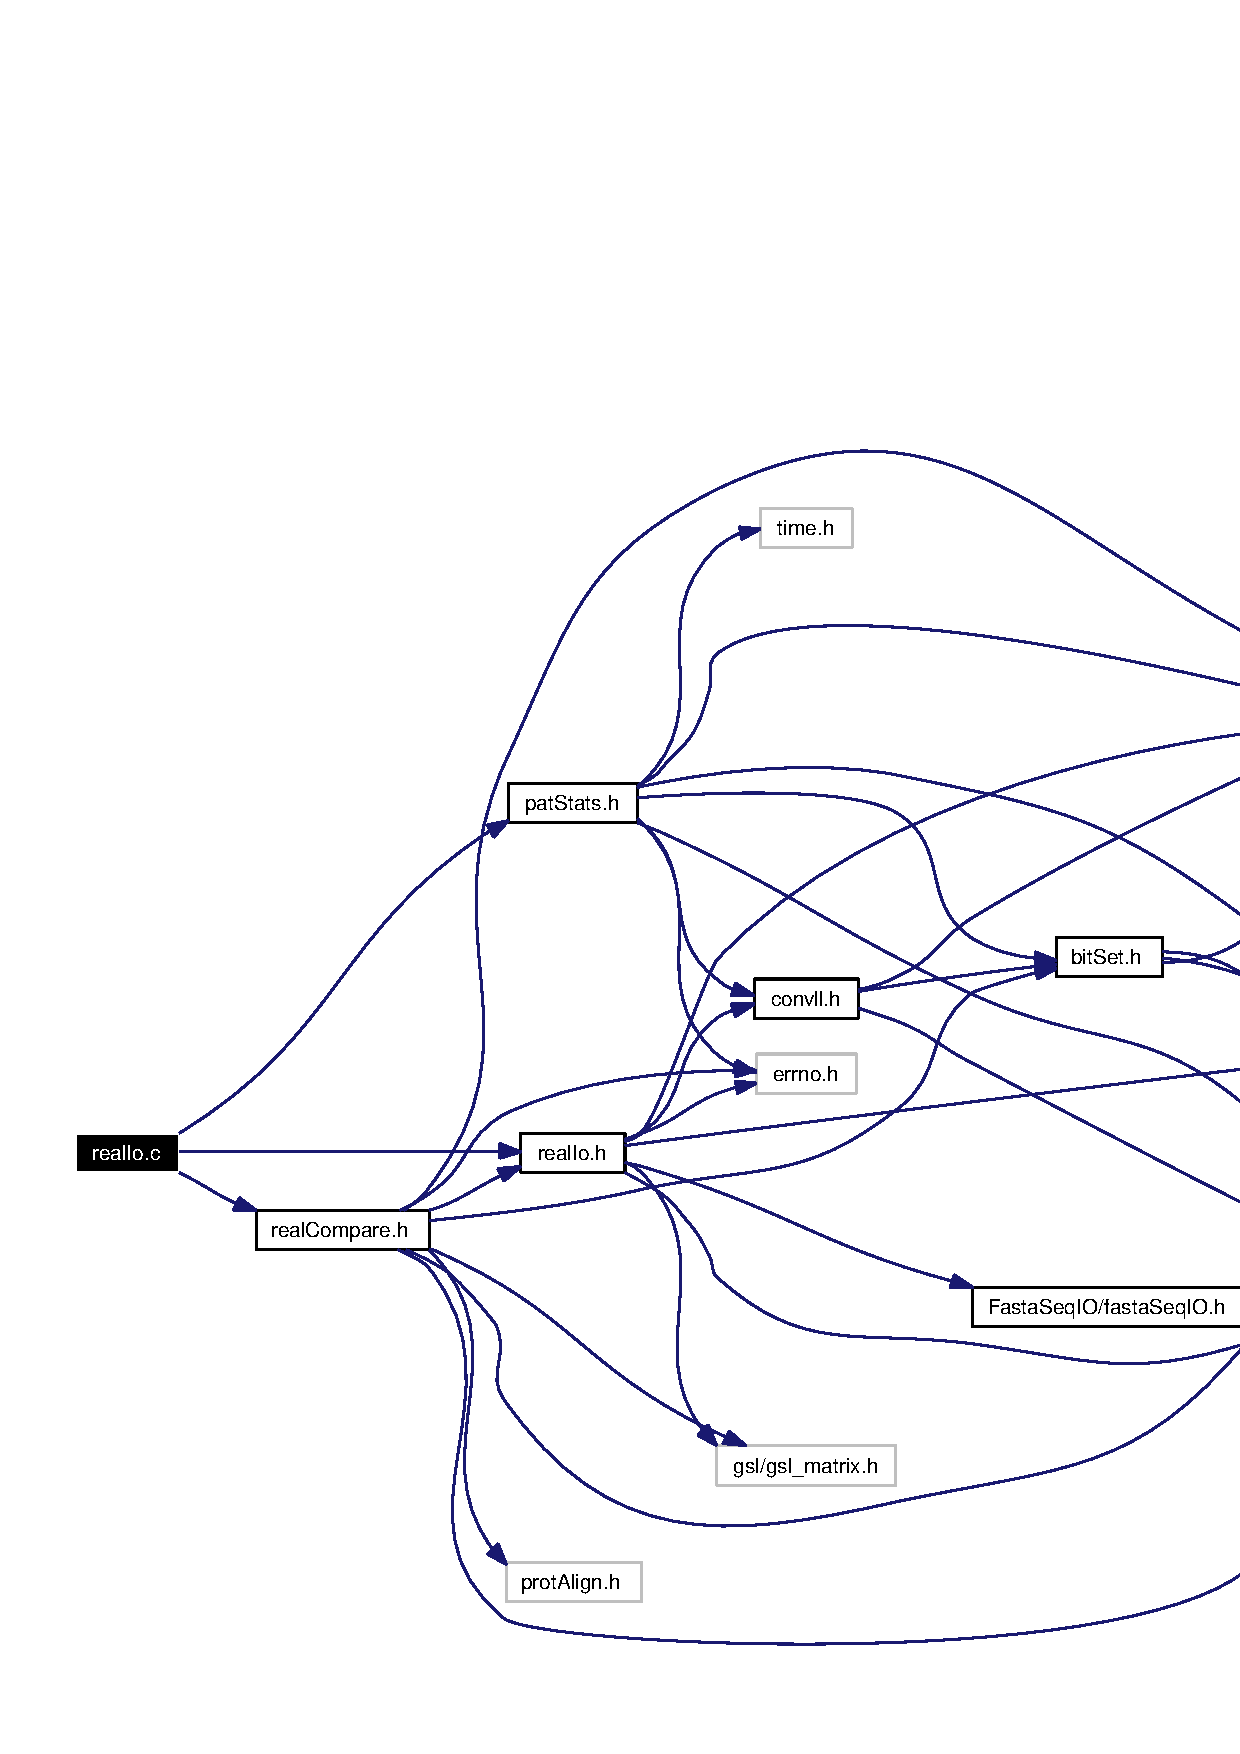
\includegraphics[width=342pt]{realIo_8c__incl}
\end{center}
\end{figure}
\subsection*{Functions}
\begin{CompactItemize}
\item 
\hyperlink{realIo_8c_a0}{word\-To\-Double} (char $\ast$s, int begin, int end)
\item 
int \hyperlink{realIo_8c_a1}{count\-Fields} (char $\ast$s, char sep)
\item 
int \hyperlink{realIo_8c_a2}{check\-Real\-Data\-Format} (char $\ast$$\ast$buf, int nl, char sep, int $\ast$num\-Seq\_\-p, int $\ast$dim\_\-p)
\item 
int \hyperlink{realIo_8c_a3}{count\-Total\-Fields} (char $\ast$$\ast$buf, int nl, char sep)
\item 
\hyperlink{structrdh__t}{rdh\_\-t} $\ast$ \hyperlink{realIo_8c_a4}{init\-Rdh} (int x)
\item 
int \hyperlink{realIo_8c_a5}{get\-Rdh\-Seq\-Length} (\hyperlink{structrdh__t}{rdh\_\-t} $\ast$data, int seq\-No)
\item 
int \hyperlink{realIo_8c_a6}{init\-Rdh\-Index} (\hyperlink{structrdh__t}{rdh\_\-t} $\ast$data, int word\-Size, int seq\-Gap)
\item 
\hyperlink{structrdh__t}{rdh\_\-t} $\ast$ \hyperlink{realIo_8c_a7}{free\-Rdh} (\hyperlink{structrdh__t}{rdh\_\-t} $\ast$data)
\item 
int \hyperlink{realIo_8c_a8}{get\-Rdh\-Dim} (\hyperlink{structrdh__t}{rdh\_\-t} $\ast$data)
\item 
int \hyperlink{realIo_8c_a9}{set\-Rdh\-Label} (\hyperlink{structrdh__t}{rdh\_\-t} $\ast$data, int seq\-No, char $\ast$s)
\item 
int \hyperlink{realIo_8c_a10}{set\-Rdh\-Value} (\hyperlink{structrdh__t}{rdh\_\-t} $\ast$data, int seq\-No, int pos\-No, int dim\-No, double val)
\item 
int \hyperlink{realIo_8c_a11}{set\-Rdh\-Index} (\hyperlink{structrdh__t}{rdh\_\-t} $\ast$data, int seq\-No, int pos\-No, int index)
\item 
int \hyperlink{realIo_8c_a12}{get\-Rdh\-Index\-Seq\-Pos} (\hyperlink{structrdh__t}{rdh\_\-t} $\ast$data, int index, int $\ast$seq, int $\ast$pos)
\item 
double \hyperlink{realIo_8c_a13}{get\-Rdh\-Value} (\hyperlink{structrdh__t}{rdh\_\-t} $\ast$data, int seq\-No, int pos\-No, int dim\-No)
\item 
char $\ast$ \hyperlink{realIo_8c_a14}{get\-Rdh\-Label} (\hyperlink{structrdh__t}{rdh\_\-t} $\ast$data, int seq\-No)
\item 
int \hyperlink{realIo_8c_a15}{print\-Rdh\-Seq} (\hyperlink{structrdh__t}{rdh\_\-t} $\ast$data, int seq\-No, FILE $\ast$FH)
\item 
int \hyperlink{realIo_8c_a16}{set\-Rdh\-Col\-From\-String} (\hyperlink{structrdh__t}{rdh\_\-t} $\ast$data, int seq\-No, int col\-No, char $\ast$s, char sep)
\item 
int \hyperlink{realIo_8c_a17}{init\-Rdh\-Gsl\-Mat} (\hyperlink{structrdh__t}{rdh\_\-t} $\ast$data, int seq\-No, int x, int y)
\item 
int \hyperlink{realIo_8c_a18}{push\-On\-Rdh\-Seq} (\hyperlink{structrdh__t}{rdh\_\-t} $\ast$data, char $\ast$$\ast$buf, int start\-Line, int dim, char sep)
\item 
\hyperlink{structrdh__t}{rdh\_\-t} $\ast$ \hyperlink{realIo_8c_a19}{parse\-Real\-Data} (char $\ast$$\ast$buf, int nl, char sep, int num\-Seq, int dim)
\item 
\hyperlink{structrdh__t}{rdh\_\-t} $\ast$ \hyperlink{realIo_8c_a20}{read\-Real\-Data} (FILE $\ast$INPUT)
\item 
int \hyperlink{realIo_8c_a21}{output\-Real\-Pats} (\hyperlink{structrdh__t}{rdh\_\-t} $\ast$data, \hyperlink{structcnode}{cll\_\-t} $\ast$all\-Pats, int L, FILE $\ast$OUTPUT\_\-FILE, int $\ast$$\ast$d)
\item 
int \hyperlink{realIo_8c_a22}{find\-Clique\-Centroid} (\hyperlink{structrdh__t}{rdh\_\-t} $\ast$data, \hyperlink{structcnode}{cll\_\-t} $\ast$cur\-Cliq, int L, int comp\-Func, double $\ast$extra\-Params, int $\ast$candidates)
\item 
int \hyperlink{realIo_8c_a23}{make\-Alternate\-Centroid} (\hyperlink{structrdh__t}{rdh\_\-t} $\ast$data, \hyperlink{structcnode}{cll\_\-t} $\ast$cur\-Cliq, int $\ast$candidates)
\item 
int \hyperlink{realIo_8c_a24}{output\-Real\-Pats\-WCentroid} (\hyperlink{structrdh__t}{rdh\_\-t} $\ast$data, \hyperlink{structcnode}{cll\_\-t} $\ast$all\-Pats, int L, FILE $\ast$OUTPUT\_\-FILE, double $\ast$extra\-Params, int comp\-Func)
\end{CompactItemize}


\subsection*{Detailed Description}
This file defines functions that are used for the parsing of user supplied data in the real valued implementation of Gemoda.

Definition in file \hyperlink{realIo_8c-source}{real\-Io.c}.

\subsection*{Function Documentation}
\hypertarget{realIo_8c_a2}{
\index{realIo.c@{real\-Io.c}!checkRealDataFormat@{checkRealDataFormat}}
\index{checkRealDataFormat@{checkRealDataFormat}!realIo.c@{real\-Io.c}}
\subsubsection[checkRealDataFormat]{\setlength{\rightskip}{0pt plus 5cm}int check\-Real\-Data\-Format (char $\ast$$\ast$ {\em buf}, int {\em nl}, char {\em sep}, int $\ast$ {\em num\-Seq\_\-p}, int $\ast$ {\em dim\_\-p})}}
\label{realIo_8c_a2}


Check that each sequence has the same dimensionality and that, within a sequence, each dimension has the same number of entries. Note: this routine alters $\ast$nun\-Seq\_\-p and $\ast$dim\_\-p! Also, you must call this routine before calling parse\-Real\-Data. Otherwise, parse\-Real\-Data is garunteed to die if the data turn out to be ill-formatted.

Definition at line 163 of file real\-Io.c.

References count\-Fields().

Referenced by read\-Real\-Data().

\scriptsize\begin{verbatim}164 {
165   int i;
166   int thisDim = 0;
167   int status = 1;
168   int width;
169   int fieldCount = 0;       // number of positions in a single sequence
170   int numSeq = 0;       // number of sequences 
171   int dim = 0;          // The dimensionality of the sequences
172 
173   // NOTE this is not checking the dimensionality of the last sequence...
174   // that's bad.  We can fix that though.
175   // Check the dimensionality of each sequence
176   for (i = 0; i < nl; i++)
177     {
178       if (buf[i][0] == '>')
179     {
180 
181       // If this is only the second sequence we've seen,
182       // record the dimensionality of the first sequence
183       // as the dim to insist upon from here on out
184       if (numSeq == 1)
185         {
186           dim = thisDim;
187 
188           // For other sequences, we need to check to make sure
189           // that they've got the same dimensions as previous
190           // sequences
191         }
192       else if (numSeq > 1)
193         {
194 
195           // If the dimensions are wrong, quit with status=0
196           if (thisDim != dim)
197         {
198           status = 0;
199           break;
200         }
201         }
202       numSeq++;
203       width = 0;
204       thisDim = 0;
205     }
206       else
207     {
208 
209       // Field count can be different for each sequence but
210       // must be the same for each dimension in a single sequence
211       fieldCount = countFields (buf[i], sep);
212 
213       // If this is the first row of this sequence,
214       // then store the number of fields
215       if (thisDim == 0)
216         {
217           width = fieldCount;
218 
219           // If it's not the first row, make sure it has the
220           // same number of fields as previous rows in this
221           // sequence
222         }
223       else
224         {
225           if (fieldCount != width)
226         {
227           status = 0;
228           break;
229         }
230         }
231       thisDim++;
232     }
233     }
234 
235   // Pass back the numSeq and dim
236   *numSeq_p = numSeq;
237   *dim_p = thisDim;
238   return status;
239 }
\end{verbatim}
\normalsize 


\hypertarget{realIo_8c_a1}{
\index{realIo.c@{real\-Io.c}!countFields@{countFields}}
\index{countFields@{countFields}!realIo.c@{real\-Io.c}}
\subsubsection[countFields]{\setlength{\rightskip}{0pt plus 5cm}int count\-Fields (char $\ast$ {\em s}, char {\em sep})}}
\label{realIo_8c_a1}


Count the number of fields (delimited by 'sep') in a single string. I was going to use strsep in string.h for this; however, I don't like that it changes the input string, which makes free-ing the string later more tricky. Ignores consecutive seperators.

Definition at line 90 of file real\-Io.c.

References word\-To\-Double().

Referenced by check\-Real\-Data\-Format(), count\-Total\-Fields(), and push\-On\-Rdh\-Seq().

\scriptsize\begin{verbatim}91 {
92   int i;
93   int begin = 0;
94   int end = 0;
95   int status = 0;       // 0 = in sep, 1 = in word
96   int fieldCount = 0;
97   double val;
98   if (s == NULL)
99     {
100       fprintf (stderr, "Passed NULL string to countFields -- error!");
101       fflush (stderr);
102       exit (0);
103     }
104 
105   // Loop over the length of the string
106   for (i = 0; i < strlen (s); i++)
107     {
108 
109       // The previous state was space
110       if (status == 0)
111     {
112 
113       // We hit a word
114       if (s[i] != sep)
115         {
116           begin = i;
117           status = 1;
118         }
119       else
120         {           // We hit more space
121           continue;
122         }
123     }
124       else
125     {           // The previous state was word
126       if (s[i] != sep)
127         {
128           continue;
129         }
130       else
131         {           // We hit a space
132           end = i - 1;
133           status = 0;
134 
135           // being and end now delimit a word,
136           // turn that word into a double
137           val = wordToDouble (s, begin, end);
138           fieldCount++;
139         }
140     }
141     }
142 
143   // At the end, if we were in a word, we have
144   // one more field
145   if (status == 1)
146     {               // We're in a word
147       val = wordToDouble (s, begin, strlen (s));
148       fieldCount++;
149     }
150   return fieldCount;
151 }
\end{verbatim}
\normalsize 


\hypertarget{realIo_8c_a3}{
\index{realIo.c@{real\-Io.c}!countTotalFields@{countTotalFields}}
\index{countTotalFields@{countTotalFields}!realIo.c@{real\-Io.c}}
\subsubsection[countTotalFields]{\setlength{\rightskip}{0pt plus 5cm}int count\-Total\-Fields (char $\ast$$\ast$ {\em buf}, int {\em nl}, char {\em sep})}}
\label{realIo_8c_a3}


Count the number of fields in each sequence and return the sum of these.

Definition at line 246 of file real\-Io.c.

References count\-Fields().

Referenced by parse\-Real\-Data().

\scriptsize\begin{verbatim}247 {
248   int i = 0;
249   int totalFields = 0;
250   int seqNo = 0;
251   while (i < nl)
252     {
253 
254       // Hit a new sequence
255       if (buf[i][0] == '>')
256     {
257       seqNo++;
258 
259       // Assume that the sequence has at least
260       // one row (should have called checkRealDataFormat!
261       // and that each row has the same number of fields
262       totalFields += countFields (buf[i + 1], sep);
263     }
264       i++;
265     }
266   return totalFields;
267 }
\end{verbatim}
\normalsize 


\hypertarget{realIo_8c_a22}{
\index{realIo.c@{real\-Io.c}!findCliqueCentroid@{findCliqueCentroid}}
\index{findCliqueCentroid@{findCliqueCentroid}!realIo.c@{real\-Io.c}}
\subsubsection[findCliqueCentroid]{\setlength{\rightskip}{0pt plus 5cm}int find\-Clique\-Centroid (\hyperlink{structrdh__t}{rdh\_\-t} $\ast$ {\em data}, \hyperlink{structcnode}{cll\_\-t} $\ast$ {\em cur\-Cliq}, int {\em L}, int {\em comp\-Func}, double $\ast$ {\em extra\-Params}, int $\ast$ {\em candidates})}}
\label{realIo_8c_a22}


This function is used to find the centroid of a clique. That is, to find the center of mass.

Definition at line 1096 of file real\-Io.c.

References get\-Comp\-Func, c\-Set\_\-t::members, cnode::set, and c\-Set\_\-t::size.

Referenced by output\-Real\-Pats\-WCentroid().

\scriptsize\begin{verbatim}1098 {
1099   double (*comparisonFunc) (rdh_t *, int, int, int, double *) = NULL;
1100   int i = 0, j = 0, indmin = -1, counter = 0;
1101   double sim = 0, min = 0, flagmin = 0;
1102   double *cliqueAdjMat = NULL;
1103   cliqueAdjMat = (double *) malloc (curCliq->set->size * sizeof (double));
1104   if (cliqueAdjMat == NULL)
1105     {
1106       fprintf (stderr, "\nMemory Error\n%s\n", strerror (errno));
1107       fflush (stderr);
1108       exit (0);
1109     }
1110   for (i = 0; i < curCliq->set->size; i++)
1111     {
1112       cliqueAdjMat[i] = 0;
1113     }
1114 
1115   // We'll accumulate our comparison function values... except here
1116   // we're really assuming that we're using a match factor, with
1117   // value less than one, so that we can subtract it from one to
1118   // get a distance, and then find the centroid by identifying the
1119   // node with the smallest cumulative Euclidean distance to all
1120   // nodes.  
1121   // Note that we only need to compare each unique pair, and can apply
1122   // the results from each comparison to each member of the pair,
1123   // hence the somewhat odd indices of initiation for the for loops.
1124   comparisonFunc = getCompFunc (compFunc);
1125   for (i = 0; i < curCliq->set->size; i++)
1126     {
1127       for (j = i + 1; j < curCliq->set->size; j++)
1128     {
1129       sim =
1130         comparisonFunc (data, curCliq->set->members[i],
1131                 curCliq->set->members[j], L, extraParams);
1132 
1133       // printf("i = %d, j = %d, L = %d, extra = %lf, sim =
1134       // %lf\n",i,j,L,extraParams[0],sim);
1135       cliqueAdjMat[i] += pow (1 - sim, 2);
1136       cliqueAdjMat[j] += pow (1 - sim, 2);
1137     }
1138     }
1139 
1140   // Now we find the minimum Euclidean distance.
1141   min = cliqueAdjMat[0];
1142   indmin = 0;
1143   for (i = 1; i < curCliq->set->size; i++)
1144     {
1145 
1146       // printf("index %d product = %lf\n",i,cliqueAdjMat[i]);
1147       if (cliqueAdjMat[i] < min)
1148     {
1149       indmin = i;
1150       min = cliqueAdjMat[i];
1151       flagmin = 0;
1152     }
1153       else if (cliqueAdjMat[i] == min)
1154     {
1155       flagmin = 1;
1156     }
1157     }
1158 
1159   // If we had a duplicate on the minimum, we locate all duplicates.
1160   if (flagmin == 1)
1161     {
1162       counter = 0;
1163       for (i = 0; i < curCliq->set->size; i++)
1164     {
1165       if (cliqueAdjMat[i] == min)
1166         {
1167           counter++;
1168           candidates[counter] = i;
1169         }
1170     }
1171 
1172       // Store the number of candidates at the array's beginning
1173       candidates[0] = counter;
1174       free (cliqueAdjMat);
1175       return (-1);
1176     }
1177   else
1178     {
1179       free (cliqueAdjMat);
1180       return (indmin);
1181     }
1182 }
\end{verbatim}
\normalsize 


\hypertarget{realIo_8c_a7}{
\index{realIo.c@{real\-Io.c}!freeRdh@{freeRdh}}
\index{freeRdh@{freeRdh}!realIo.c@{real\-Io.c}}
\subsubsection[freeRdh]{\setlength{\rightskip}{0pt plus 5cm}\hyperlink{structrdh__t}{rdh\_\-t}$\ast$ free\-Rdh (\hyperlink{structrdh__t}{rdh\_\-t} $\ast$ {\em data})}}
\label{realIo_8c_a7}


This function returns a null pointer after freeing the memory associated with a real data holder object. The function takes one parameter: a pointer to the real data holder, {\em data\/}.

Definition at line 462 of file real\-Io.c.

References rdh\_\-t::index\-To\-Pos, rdh\_\-t::index\-To\-Seq, rdh\_\-t::label, rdh\_\-t::offset\-To\-Index, and rdh\_\-t::seq.

Referenced by main().

\scriptsize\begin{verbatim}463 {
464   int i;
465   if (data != NULL)
466     {
467       if (data->indexToPos != NULL)
468     {
469       free (data->indexToPos);
470       data->indexToPos = NULL;
471     }
472       if (data->indexToSeq != NULL)
473     {
474       free (data->indexToSeq);
475       data->indexToSeq = NULL;
476     }
477       if (data->offsetToIndex != NULL)
478     {
479       for (i = 0; i < data->size; i++)
480         {
481           free (data->offsetToIndex[i]);
482           data->offsetToIndex[i] = NULL;
483         }
484       free (data->offsetToIndex);
485       data->offsetToIndex = NULL;
486     }
487       for (i = 0; i < data->size; i++)
488     {
489       if (data->seq[i] != NULL)
490         {
491           gsl_matrix_free (data->seq[i]);
492           data->seq[i] = NULL;
493         }
494       if (data->label[i] != NULL)
495         {
496           free (data->label[i]);
497           data->label[i] = NULL;
498         }
499     }
500       if (data->seq != NULL)
501     {
502       free (data->seq);
503       data->seq = NULL;
504     }
505       if (data->label != NULL)
506     {
507       free (data->label);
508       data->label = NULL;
509     }
510       free (data);
511       data = NULL;
512     }
513   return data;
514 }
\end{verbatim}
\normalsize 


\hypertarget{realIo_8c_a8}{
\index{realIo.c@{real\-Io.c}!getRdhDim@{getRdhDim}}
\index{getRdhDim@{getRdhDim}!realIo.c@{real\-Io.c}}
\subsubsection[getRdhDim]{\setlength{\rightskip}{0pt plus 5cm}int get\-Rdh\-Dim (\hyperlink{structrdh__t}{rdh\_\-t} $\ast$ {\em data})}}
\label{realIo_8c_a8}


This function returns an integer equal to the dimensions of the data stored in a real data holder object. The function takes one parameter: a pointer to the real data holder, {\em data\/}.

Definition at line 524 of file real\-Io.c.

References rdh\_\-t::seq.

Referenced by general\-Match\-Factor(), get\-Rdh\-Value(), mass\-Spec\-Compare\-WElut(), print\-Rdh\-Seq(), rmsd\-Compare(), and set\-Rdh\-Value().

\scriptsize\begin{verbatim}525 {
526   if (data == NULL || data->seq == NULL || data->seq[0] == NULL)
527     {
528       fprintf (stderr, "Passed bad data to getRdhSeqLength -- error!");
529       fflush (stderr);
530       exit (0);
531     }
532   return data->seq[0]->size2;
533 }
\end{verbatim}
\normalsize 


\hypertarget{realIo_8c_a12}{
\index{realIo.c@{real\-Io.c}!getRdhIndexSeqPos@{getRdhIndexSeqPos}}
\index{getRdhIndexSeqPos@{getRdhIndexSeqPos}!realIo.c@{real\-Io.c}}
\subsubsection[getRdhIndexSeqPos]{\setlength{\rightskip}{0pt plus 5cm}int get\-Rdh\-Index\-Seq\-Pos (\hyperlink{structrdh__t}{rdh\_\-t} $\ast$ {\em data}, int {\em index}, int $\ast$ {\em seq}, int $\ast$ {\em pos})}}
\label{realIo_8c_a12}


This function is used to access and change the sequence and position values, given an index. The function takes four parameters: a pointer to the real data holder, {\em data\/}, an integer {\em index\/}, a pointer integer {\em seq\/}, and a pointer integer {\em pos\/}.

Definition at line 633 of file real\-Io.c.

References rdh\_\-t::index\-Size, rdh\_\-t::index\-To\-Pos, and rdh\_\-t::index\-To\-Seq.

Referenced by general\-Match\-Factor(), make\-Alternate\-Centroid(), mass\-Spec\-Compare\-WElut(), output\-Real\-Pats(), output\-Real\-Pats\-WCentroid(), real\-Comparison(), and rmsd\-Compare().

\scriptsize\begin{verbatim}634 {
635   if (data == NULL || data->indexToSeq == NULL || data->indexToPos == NULL
636       || index > data->indexSize)
637     {
638       fprintf (stderr, "Passed bad data to getRdhIndexSeqPos -- error!");
639       fflush (stderr);
640       exit (0);
641     }
642 
643   /*
644      printf("Setting index %d -> %d, %d\n", index, seqNo, posNo);
645    */
646   /*
647      fflush(stdout);
648    */
649   *seq = data->indexToSeq[index];
650   *pos = data->indexToPos[index];
651   return 0;
652 }
\end{verbatim}
\normalsize 


\hypertarget{realIo_8c_a14}{
\index{realIo.c@{real\-Io.c}!getRdhLabel@{getRdhLabel}}
\index{getRdhLabel@{getRdhLabel}!realIo.c@{real\-Io.c}}
\subsubsection[getRdhLabel]{\setlength{\rightskip}{0pt plus 5cm}char$\ast$ get\-Rdh\-Label (\hyperlink{structrdh__t}{rdh\_\-t} $\ast$ {\em data}, int {\em seq\-No})}}
\label{realIo_8c_a14}


This function is used to retrieve the label of a particular sequence in a real data holder object. The function takes two parameters: a pointer to the real data holder {\em data\/}; and an integer which is the sequence number to be accessed {\em seq\-No\/}. The function returns a pointer to a string, which is the label for that sequence.

Definition at line 689 of file real\-Io.c.

References rdh\_\-t::label.

Referenced by print\-Rdh\-Seq().

\scriptsize\begin{verbatim}690 {
691   if (data == NULL || data->label == NULL || data->label[seqNo] == NULL)
692     {
693       fprintf (stderr, "Passed bad data to getRdhLabel -- error!");
694       fflush (stderr);
695       exit (0);
696     }
697   return data->label[seqNo];
698 }
\end{verbatim}
\normalsize 


\hypertarget{realIo_8c_a5}{
\index{realIo.c@{real\-Io.c}!getRdhSeqLength@{getRdhSeqLength}}
\index{getRdhSeqLength@{getRdhSeqLength}!realIo.c@{real\-Io.c}}
\subsubsection[getRdhSeqLength]{\setlength{\rightskip}{0pt plus 5cm}int get\-Rdh\-Seq\-Length (\hyperlink{structrdh__t}{rdh\_\-t} $\ast$ {\em data}, int {\em seq\-No})}}
\label{realIo_8c_a5}


This function returns an integer that is equal to the sequence length of a particular sequence within the real data holder object. The function takes two parameters: a pointer to the real data holder, {\em data\/}, and the index of the sequence for which we need to know the length, {\em seq\-No\/}.

Definition at line 331 of file real\-Io.c.

References rdh\_\-t::seq.

Referenced by get\-Rdh\-Value(), init\-Rdh\-Index(), print\-Rdh\-Seq(), and set\-Rdh\-Value().

\scriptsize\begin{verbatim}332 {
333   if (data == NULL || data->seq == NULL || data->seq[seqNo] == NULL)
334     {
335       fprintf (stderr, "Passed bad data to getRdhSeqLength -- error!");
336       fflush (stderr);
337       exit (0);
338     }
339   return data->seq[seqNo]->size1;
340 }
\end{verbatim}
\normalsize 


\hypertarget{realIo_8c_a13}{
\index{realIo.c@{real\-Io.c}!getRdhValue@{getRdhValue}}
\index{getRdhValue@{getRdhValue}!realIo.c@{real\-Io.c}}
\subsubsection[getRdhValue]{\setlength{\rightskip}{0pt plus 5cm}double get\-Rdh\-Value (\hyperlink{structrdh__t}{rdh\_\-t} $\ast$ {\em data}, int {\em seq\-No}, int {\em pos\-No}, int {\em dim\-No})}}
\label{realIo_8c_a13}


This function is used to retrieve the value of a particular dimension, position, and sequence. The function takes four parameters: a pointer to the real data holder {\em data\/}; an integer which is the sequence number to be accessed {\em seq\-No\/}; an integer that is the position number to be accessed {\em pos\-No\/}; and an integer that is the dimension to be accessed {\em dim\-No\/}.

Definition at line 666 of file real\-Io.c.

References get\-Rdh\-Dim(), get\-Rdh\-Seq\-Length(), and rdh\_\-t::seq.

Referenced by print\-Rdh\-Seq().

\scriptsize\begin{verbatim}667 {
668   if (data == NULL || data->seq == NULL || data->seq[seqNo] == NULL
669       || posNo > getRdhSeqLength (data, seqNo) || dimNo > getRdhDim (data))
670     {
671       fprintf (stderr, "Passed bad data to getRdhValue -- error!");
672       fflush (stderr);
673       exit (0);
674     }
675   return gsl_matrix_get (data->seq[seqNo], posNo, dimNo);
676 }
\end{verbatim}
\normalsize 


\hypertarget{realIo_8c_a4}{
\index{realIo.c@{real\-Io.c}!initRdh@{initRdh}}
\index{initRdh@{initRdh}!realIo.c@{real\-Io.c}}
\subsubsection[initRdh]{\setlength{\rightskip}{0pt plus 5cm}\hyperlink{structrdh__t}{rdh\_\-t}$\ast$ init\-Rdh (int {\em x})}}
\label{realIo_8c_a4}


This function initializes a real data holder object. The function takes as its input a size {\em x\/} which is the number of sequences that will be stored in the object. The function returns a pointer to the object, which has been allocated the correct amount of memory.

Definition at line 277 of file real\-Io.c.

References rdh\_\-t::index\-Size, rdh\_\-t::index\-To\-Pos, rdh\_\-t::index\-To\-Seq, rdh\_\-t::label, rdh\_\-t::seq, and rdh\_\-t::size.

Referenced by parse\-Real\-Data().

\scriptsize\begin{verbatim}278 {
279   int i;
280   rdh_t *data = NULL;
281 
282   // Allocate space for our structure
283   data = (rdh_t *) malloc (sizeof (rdh_t));
284   if (data == NULL)
285     {
286       fprintf (stderr, "\nMemory Error\n%s\n", strerror (errno));
287       fflush (stderr);
288       exit (0);
289     }
290   data->size = x;
291 
292   // Index has to be initialized later, once
293   // we know the word size.
294   data->indexSize = 0;
295   data->indexToSeq = NULL;
296   data->indexToPos = NULL;
297 
298   /*
299      data->indexSize = y;
300    */
301   data->label = (char **) malloc (data->size * sizeof (char *));
302   if (data->label == NULL)
303     {
304       fprintf (stderr, "\nMemory Error\n%s\n", strerror (errno));
305       fflush (stderr);
306       exit (0);
307     }
308   data->seq = (gsl_matrix **) malloc (data->size * sizeof (gsl_matrix *));
309   if (data->seq == NULL)
310     {
311       fprintf (stderr, "\nMemory Error\n%s\n", strerror (errno));
312       fflush (stderr);
313       exit (0);
314     }
315   for (i = 0; i < data->size; i++)
316     {
317       data->label[i] = NULL;
318       data->seq[i] = NULL;
319     }
320   return data;
321 }
\end{verbatim}
\normalsize 


\hypertarget{realIo_8c_a17}{
\index{realIo.c@{real\-Io.c}!initRdhGslMat@{initRdhGslMat}}
\index{initRdhGslMat@{initRdhGslMat}!realIo.c@{real\-Io.c}}
\subsubsection[initRdhGslMat]{\setlength{\rightskip}{0pt plus 5cm}int init\-Rdh\-Gsl\-Mat (\hyperlink{structrdh__t}{rdh\_\-t} $\ast$ {\em data}, int {\em seq\-No}, int {\em x}, int {\em y})}}
\label{realIo_8c_a17}


This function is used to initialize the memory for the matrix in which the real value to data are stored. To store these data, we use the GNU scientific library. The function takes four parameters: a pointer to the real data holder {\em data\/}; an integer, which is the sequence number to be set {\em seq\-No\/}; an integer, which is the first dimension of the matrix size {\em x\/}; and an integer, which is the second dimension of the matrix size {\em y\/};

Definition at line 829 of file real\-Io.c.

References rdh\_\-t::seq.

Referenced by push\-On\-Rdh\-Seq().

\scriptsize\begin{verbatim}830 {
831   data->seq[seqNo] = gsl_matrix_alloc (x, y);
832   if (data->seq[seqNo] == NULL)
833     {
834       return 0;
835     }
836   else
837     {
838       return 1;
839     }
840 }
\end{verbatim}
\normalsize 


\hypertarget{realIo_8c_a6}{
\index{realIo.c@{real\-Io.c}!initRdhIndex@{initRdhIndex}}
\index{initRdhIndex@{initRdhIndex}!realIo.c@{real\-Io.c}}
\subsubsection[initRdhIndex]{\setlength{\rightskip}{0pt plus 5cm}int init\-Rdh\-Index (\hyperlink{structrdh__t}{rdh\_\-t} $\ast$ {\em data}, int {\em word\-Size}, int {\em seq\-Gap})}}
\label{realIo_8c_a6}


This function is used to initialize the two indices inside a real data holder. The function takes as its input three parameters a pointer to the real data holder, {\em data\/}, the size of the words to be compared during the comparison stage {\em word\-Size\/}, and an integer {\em seq\-Gap\/}, which is used to place empty data between unique sequences, such that we do not convolve from one sequence into another during the convolution stage.

Definition at line 358 of file real\-Io.c.

References get\-Rdh\-Seq\-Length(), rdh\_\-t::index\-Size, rdh\_\-t::index\-To\-Pos, rdh\_\-t::index\-To\-Seq, rdh\_\-t::offset\-To\-Index, and rdh\_\-t::size.

Referenced by real\-Comparison().

\scriptsize\begin{verbatim}359 {
360   int i, j, k;
361   int numWindows = 0;
362   int thisNumWindows;
363   int numSeq;
364   int seqLen = 0;
365 
366   // The number of sequences
367   numSeq = data->size;
368 
369   // Allocate offsetToIndex's outer structure
370   data->offsetToIndex = (int **) malloc (numSeq * sizeof (int *));
371   if (data->offsetToIndex == NULL)
372     {
373       fprintf (stderr, "\nMemory Error\n%s\n", strerror (errno));
374       fflush (stderr);
375       exit (0);
376     }
377 
378   // For each sequence
379   for (i = 0; i < numSeq; i++)
380     {
381 
382       // How many windows are in this sequence
383       seqLen = getRdhSeqLength (data, i);
384       numWindows += seqLen - wordSize + 1;
385 
386       // And also use this to further allocate offsetToIndex
387       data->offsetToIndex[i] =
388     (int *) malloc ((seqLen - wordSize + 1) * sizeof (int));
389       if (data->offsetToIndex[i] == NULL)
390     {
391       fprintf (stderr, "\nMemory Error\n%s\n", strerror (errno));
392       fflush (stderr);
393       exit (0);
394     }
395     }
396 
397   // One index for each word plus seqGap between each sequence
398   // and a gap at the end
399   data->indexSize = numWindows + numSeq * seqGap;
400 
401   // Allocate indexToSeq 
402   // NOTE that it should be size of int, not int *... I think we got
403   // fortunate in the previous revision because they are the same
404   // size
405   data->indexToSeq = (int *) malloc (data->indexSize * sizeof (int));
406   if (data->indexToSeq == NULL)
407     {
408       fprintf (stderr, "\nMemory Error\n%s\n", strerror (errno));
409       fflush (stderr);
410       exit (0);
411     }
412 
413   // Allocate indexToPos 
414   // See above for int vs. int* argument.
415   data->indexToPos = (int *) malloc (data->indexSize * sizeof (int));
416   if (data->indexToPos == NULL)
417     {
418       fprintf (stderr, "\nMemory Error\n%s\n", strerror (errno));
419       fflush (stderr);
420       exit (0);
421     }
422 
423   // Fill in the values
424   k = 0;
425   for (i = 0; i < numSeq; i++)
426     {
427 
428       // How many windows are in this sequence?
429       thisNumWindows = getRdhSeqLength (data, i) - wordSize + 1;
430 
431       // For each window, make an entry in the indexToSeq
432       // and indexToPos and offsetToIndex
433       for (j = 0; j < thisNumWindows; j++)
434     {
435       data->indexToSeq[k] = i;
436       data->indexToPos[k] = j;
437       data->offsetToIndex[i][j] = k;
438       k++;
439     }
440 
441       // Add gaps between sequences in the index.
442       // Usually seqGap is just 1;
443       for (j = 0; j < seqGap; j++)
444     {
445 
446       // -1 means no sequence and no position
447       data->indexToSeq[k] = -1;
448       data->indexToPos[k] = -1;
449       k++;
450     }
451     }
452   return 0;
453 }
\end{verbatim}
\normalsize 


\hypertarget{realIo_8c_a23}{
\index{realIo.c@{real\-Io.c}!makeAlternateCentroid@{makeAlternateCentroid}}
\index{makeAlternateCentroid@{makeAlternateCentroid}!realIo.c@{real\-Io.c}}
\subsubsection[makeAlternateCentroid]{\setlength{\rightskip}{0pt plus 5cm}int make\-Alternate\-Centroid (\hyperlink{structrdh__t}{rdh\_\-t} $\ast$ {\em data}, \hyperlink{structcnode}{cll\_\-t} $\ast$ {\em cur\-Cliq}, int $\ast$ {\em candidates})}}
\label{realIo_8c_a23}


This function is used to choose an alternate centroid for a given clique. In order to make the centroid decision slightly less dependent on input order, we decide to choose from the tied candidates the one whose relative position in the sequence is highest. There is no basis in theory for this, it is done so that a consistent choice is made. Only rarely will two spectra be tied for being a centroid and have the same sequence number. In that case, we pretty much have to default to the sequence number, which is what would be done without this function. Note that now though we are less sensitive to the order of input of the sequences, we are now more sensitive to the context surrounding a given spectrum. That is, if it is put in the beginning of the sequence, it is more likely to be chosen. This choice can only be justified insofar as if multiple choices are tied, then they are the same cumulative distance to the clique, and so $\ast$any$\ast$ should be allowed to be chosen equally. There should be little difference in terms of tangible results. This just makes the semantics consistent.

Definition at line 1202 of file real\-Io.c.

References get\-Rdh\-Index\-Seq\-Pos(), c\-Set\_\-t::members, and cnode::set.

Referenced by output\-Real\-Pats\-WCentroid().

\scriptsize\begin{verbatim}1203 {
1204   int indmin, min, i;
1205   int curSeq, curPos;
1206   int numCandidates = candidates[0];
1207   indmin = candidates[1];
1208   getRdhIndexSeqPos (data, curCliq->set->members[indmin], &curSeq, &curPos);
1209   min = curPos;
1210 
1211   // We use less-than-or-equal here because we're starting at 1, 
1212   // so we want 1 to end.  The length of candidates is one more than
1213   // the maxSup, so we know we can reach candidates[maxSup] without
1214   // a segfault.
1215   for (i = 2; i <= numCandidates; i++)
1216     {
1217       getRdhIndexSeqPos (data, curCliq->set->members[candidates[i]], &curSeq,
1218              &curPos);
1219       if (curPos < min)
1220     {
1221       indmin = candidates[i];
1222       min = curPos;
1223     }
1224     }
1225   return (indmin);
1226 }
\end{verbatim}
\normalsize 


\hypertarget{realIo_8c_a21}{
\index{realIo.c@{real\-Io.c}!outputRealPats@{outputRealPats}}
\index{outputRealPats@{outputRealPats}!realIo.c@{real\-Io.c}}
\subsubsection[outputRealPats]{\setlength{\rightskip}{0pt plus 5cm}int output\-Real\-Pats (\hyperlink{structrdh__t}{rdh\_\-t} $\ast$ {\em data}, \hyperlink{structcnode}{cll\_\-t} $\ast$ {\em all\-Pats}, int {\em L}, FILE $\ast$ {\em OUTPUT\_\-FILE}, int $\ast$$\ast$ {\em d})}}
\label{realIo_8c_a21}


This function is used to print out motifs discovered by Gemoda in an attractive fashion. The function takes five parameters: a pointer to a real data holder object {\em data\/}; a pointer to a linked list of motifs {\em all\-Pats\/}; an integer which is Gemoda's input parameter {\em L\/}; and a pointer to a file handle to which output is printed {\em OUTPUT\_\-FILE\/}.

Definition at line 1046 of file real\-Io.c.

References get\-Rdh\-Index\-Seq\-Pos(), cnode::length, c\-Set\_\-t::members, cnode::next, rdh\_\-t::seq, cnode::set, c\-Set\_\-t::size, and cnode::stat.

Referenced by main().

\scriptsize\begin{verbatim}1048 {
1049   int i, j, pos1;
1050   int curSeq, curPos;
1051   cll_t *curCliq = NULL;
1052   curCliq = allPats;
1053   i = 0;
1054   while (curCliq != NULL)
1055     {
1056       fprintf (OUTPUT_FILE, "pattern %d:\tlen=%d\tsup=%d\t", i,
1057            curCliq->length + L, curCliq->set->size);
1058       if (d != NULL)
1059     {
1060       fprintf (OUTPUT_FILE, "\tsignif=%le\n", curCliq->stat);
1061     }
1062       else
1063     {
1064       fprintf (OUTPUT_FILE, "\n");
1065     }
1066       for (j = 0; j < curCliq->set->size; j++)
1067     {
1068       pos1 = curCliq->set->members[j];
1069       getRdhIndexSeqPos (data, pos1, &curSeq, &curPos);
1070       fprintf (OUTPUT_FILE, "   %d\t%d\t", curSeq, curPos);
1071       fprintf (OUTPUT_FILE, "%lf\t",
1072            gsl_matrix_get (data->seq[curSeq], curPos, 0));
1073 
1074       /*
1075          for(k=curPos ; k<curPos+curCliq->length+L ; k++){ fprintf(OUTPUT_FILE, "%c",
1076          mySequences[curSeq].seq[k]); } 
1077        */
1078       fprintf (OUTPUT_FILE, "\n");
1079     }
1080       fprintf (OUTPUT_FILE, "\n\n");
1081       curCliq = curCliq->next;
1082       i++;
1083     }
1084   return 0;
1085 }
\end{verbatim}
\normalsize 


\hypertarget{realIo_8c_a24}{
\index{realIo.c@{real\-Io.c}!outputRealPatsWCentroid@{outputRealPatsWCentroid}}
\index{outputRealPatsWCentroid@{outputRealPatsWCentroid}!realIo.c@{real\-Io.c}}
\subsubsection[outputRealPatsWCentroid]{\setlength{\rightskip}{0pt plus 5cm}int output\-Real\-Pats\-WCentroid (\hyperlink{structrdh__t}{rdh\_\-t} $\ast$ {\em data}, \hyperlink{structcnode}{cll\_\-t} $\ast$ {\em all\-Pats}, int {\em L}, FILE $\ast$ {\em OUTPUT\_\-FILE}, double $\ast$ {\em extra\-Params}, int {\em comp\-Func})}}
\label{realIo_8c_a24}


This function is used to output real valued patterns in a format such that they are centered on a particular centroid.

Definition at line 1233 of file real\-Io.c.

References find\-Clique\-Centroid(), get\-Comp\-Func, get\-Rdh\-Index\-Seq\-Pos(), cnode::length, make\-Alternate\-Centroid(), c\-Set\_\-t::members, cnode::next, cnode::set, and c\-Set\_\-t::size.

Referenced by main().

\scriptsize\begin{verbatim}1236 {
1237   int i, j, k, pos1, centroid;
1238   int curSeq, curPos;
1239   int maxSup = 0;
1240   cll_t *curCliq = NULL;
1241   double mfToCentroid = 0;
1242   double (*comparisonFunc) (rdh_t *, int, int, int, double *) = NULL;
1243   int *candidates = NULL;
1244   curCliq = allPats;
1245   while (curCliq != NULL)
1246     {
1247       if (curCliq->set->size > maxSup)
1248     {
1249       maxSup = curCliq->set->size;
1250     }
1251       curCliq = curCliq->next;
1252     }
1253   candidates = (int *) malloc ((maxSup + 1) * sizeof (int));
1254   if (candidates == NULL)
1255     {
1256       fprintf (stderr, "\nMemory Error\n%s\n", strerror (errno));
1257       fflush (stderr);
1258       exit (0);
1259     }
1260   for (i = 0; i <= maxSup; i++)
1261     {
1262       candidates[i] = 0;
1263     }
1264   comparisonFunc = getCompFunc (compFunc);
1265   curCliq = allPats;
1266   i = 0;
1267   while (curCliq != NULL)
1268     {
1269       fprintf (OUTPUT_FILE, "pattern %d:\tlen=%d\tsup=%d\n", i,
1270            curCliq->length + L, curCliq->set->size);
1271       centroid =
1272     findCliqueCentroid (data, curCliq, L, compFunc, extraParams,
1273                 candidates);
1274       if (centroid < 0)
1275     {
1276       centroid = makeAlternateCentroid (data, curCliq, candidates);
1277 
1278       // fprintf(OUTPUT_FILE, "WARNING: No single node in"
1279       // " cluster has non-zero similarity to all other\n nodes"
1280       // " in cluster; centroid set to first node.\n");
1281       // centroid = 0;
1282     }
1283       for (j = 0; j < curCliq->set->size; j++)
1284     {
1285       pos1 = curCliq->set->members[j];
1286       getRdhIndexSeqPos (data, pos1, &curSeq, &curPos);
1287       fprintf (OUTPUT_FILE, "   %d\t%d\t", curSeq, curPos);
1288 
1289       // fprintf(OUTPUT_FILE, "%lf\t",
1290       // gsl_matrix_get(data->seq[curSeq],curPos,0));
1291       mfToCentroid =
1292         comparisonFunc (data, curCliq->set->members[j],
1293                 curCliq->set->members[centroid], L, extraParams);
1294       fprintf (OUTPUT_FILE, "%lf\t", mfToCentroid);
1295 
1296       /*
1297          for(k=curPos ; k<curPos+curCliq->length+L ; k++){ fprintf(OUTPUT_FILE, "%c",
1298          mySequences[curSeq].seq[k]); } 
1299        */
1300       fprintf (OUTPUT_FILE, "\n");
1301     }
1302       fprintf (OUTPUT_FILE, "\n\n");
1303       curCliq = curCliq->next;
1304       i++;
1305       for (k = 0; k <= maxSup; k++)
1306     {
1307       candidates[k] = 0;
1308     }
1309     }
1310   free (candidates);
1311   return 0;
1312 }
\end{verbatim}
\normalsize 


\hypertarget{realIo_8c_a19}{
\index{realIo.c@{real\-Io.c}!parseRealData@{parseRealData}}
\index{parseRealData@{parseRealData}!realIo.c@{real\-Io.c}}
\subsubsection[parseRealData]{\setlength{\rightskip}{0pt plus 5cm}\hyperlink{structrdh__t}{rdh\_\-t}$\ast$ parse\-Real\-Data (char $\ast$$\ast$ {\em buf}, int {\em nl}, char {\em sep}, int {\em num\-Seq}, int {\em dim})}}
\label{realIo_8c_a19}


This function is used to parse a single line of a fast\-A formatted input buffer containing real valued data. The function takes

parameters: a pointer to an array of pointers to characters, which stores the sequences that we will read from {\em buf\/}; an integer, which is the line in the buffer on which we should start {\em nl\/}; a single character, which is used to delimit the input data {\em sep\/}; an integer which is the number of the sequence that we are currently reading in {\em num\-Seq\/}; an integer that is the dimensionality of the input data {\em dim\/};

Definition at line 933 of file real\-Io.c.

References count\-Total\-Fields(), init\-Rdh(), and push\-On\-Rdh\-Seq().

Referenced by read\-Real\-Data().

\scriptsize\begin{verbatim}934 {
935   int i;
936   int seqNo = -1;
937   int totalNumFields;
938   rdh_t *data = NULL;
939   totalNumFields = countTotalFields (buf, nl, sep);
940 
941   /*
942      data = initRdh(numSeq, totalNumFields + numSeq - 1);
943    */
944   data = initRdh (numSeq);
945 
946   // We're going to add an empty index between
947   // windows that correspond to different 
948   // sequences
949 
950   // Fast forward to the first sequence
951   i = 0;
952   while (i < nl)
953     {
954 
955       // Hit a new sequence
956       if (buf[i][0] == '>')
957     {
958       seqNo++;      // Note that seqNo started at -1!
959       pushOnRdhSeq (data, buf, i, dim, sep);
960       i += dim + 1;
961     }
962       else
963     {
964       i++;
965     }
966     }
967 
968   /*
969      printRdhSeq(data, 0, stdout);
970    */
971   return data;
972 }
\end{verbatim}
\normalsize 


\hypertarget{realIo_8c_a15}{
\index{realIo.c@{real\-Io.c}!printRdhSeq@{printRdhSeq}}
\index{printRdhSeq@{printRdhSeq}!realIo.c@{real\-Io.c}}
\subsubsection[printRdhSeq]{\setlength{\rightskip}{0pt plus 5cm}int print\-Rdh\-Seq (\hyperlink{structrdh__t}{rdh\_\-t} $\ast$ {\em data}, int {\em seq\-No}, FILE $\ast$ {\em FH})}}
\label{realIo_8c_a15}


This function is used to print out a real valued data sequence in a pretty manner. The function takes three parameters: a pointer to the real data holder {\em data\/}; an integer which is the sequence to be printed out {\em seq\-No\/}; and a pointer to a file handle which is where the output will be printed {\em FH\/}.

Definition at line 710 of file real\-Io.c.

References get\-Rdh\-Dim(), get\-Rdh\-Label(), get\-Rdh\-Seq\-Length(), and get\-Rdh\-Value().

\scriptsize\begin{verbatim}711 {
712   int i, j;
713   int len;
714   int dim;
715   len = getRdhSeqLength (data, seqNo);
716   dim = getRdhDim (data);
717   fprintf (FH, "%s\n", getRdhLabel (data, seqNo));
718   for (i = 0; i < len; i++)
719     {
720       for (j = 0; j < dim; j++)
721     {
722       fprintf (FH, "%3.1f ", getRdhValue (data, seqNo, i, j));
723     }
724       fprintf (FH, "\n");
725     }
726   return 0;
727 }
\end{verbatim}
\normalsize 


\hypertarget{realIo_8c_a18}{
\index{realIo.c@{real\-Io.c}!pushOnRdhSeq@{pushOnRdhSeq}}
\index{pushOnRdhSeq@{pushOnRdhSeq}!realIo.c@{real\-Io.c}}
\subsubsection[pushOnRdhSeq]{\setlength{\rightskip}{0pt plus 5cm}int push\-On\-Rdh\-Seq (\hyperlink{structrdh__t}{rdh\_\-t} $\ast$ {\em data}, char $\ast$$\ast$ {\em buf}, int {\em start\-Line}, int {\em dim}, char {\em sep})}}
\label{realIo_8c_a18}


This function is used to fill in a real data holder structure as we are reading in the sequences. Notably, this routine uses a few static variables, so it can only be called once and should not be used to alter the real data holder structure later. The function takes five parameters: a pointer to the real data holder {\em data\/}; a pointer to an array of pointers to characters, which stores the sequences that we will read from {\em buf\/}; an integer, which is the line in the buffer on which we should start {\em start\-Line\/}; an integer that is the dimensionality of the input data {\em dim\/}; a single character, which is used to delimit the input data {\em sep\/};

Definition at line 863 of file real\-Io.c.

References count\-Fields(), init\-Rdh\-Gsl\-Mat(), set\-Rdh\-Col\-From\-String(), and set\-Rdh\-Label().

Referenced by parse\-Real\-Data().

\scriptsize\begin{verbatim}864 {
865   int i, j, k;
866   int numFields;
867 
868   // NOTE THAT THESE ARE STATIC VARIABLES!!!!!
869   // That is, they retain their last value on
870   // each call to this function!
871   static int seqNo = 0;
872 
873   /*
874      static int indexNo=0;
875    */
876   i = startLine;
877 
878   // Assume that the sequence has at least
879   // one row (should have called checkRealDataFormat!
880   numFields = countFields (buf[i + 1], sep);
881 
882   // Initialize the gsl_matrix object for this 
883   // sequence in 'data'
884   // 
885   // NOTE THAT WE STORE THE TRANSPOSE OF WHAT'S IN
886   // THE INPUT FILE -- x,y = position x, dimension y
887   initRdhGslMat (data, seqNo, numFields, dim);
888 
889   // Set the sequence label
890   setRdhLabel (data, seqNo, buf[i]);
891 
892   // Read in 'dim' rows
893   for (j = i + 1, k = 0; j < i + 1 + dim; j++, k++)
894     {
895 
896       /*
897          printf("%d\n", countFields(buf[j], sep));
898        */
899 
900       // Set the k-th dimension of this sequence
901       // STILL NOTE THE TRANSPOSE!
902       setRdhColFromString (data, seqNo, k, buf[j], sep);
903     }
904 
905   /*
906      for ( l=0 ; l<numFields ; l++ ){ setRdhIndex(data, seqNo, l, indexNo); indexNo++;
907      } 
908    */
909   seqNo++;
910 
911   // Augment indexNo once more to have a -1 between each sequence!
912   /*
913      indexNo++; 
914    */
915   return 0;
916 }
\end{verbatim}
\normalsize 


\hypertarget{realIo_8c_a20}{
\index{realIo.c@{real\-Io.c}!readRealData@{readRealData}}
\index{readRealData@{readRealData}!realIo.c@{real\-Io.c}}
\subsubsection[readRealData]{\setlength{\rightskip}{0pt plus 5cm}\hyperlink{structrdh__t}{rdh\_\-t}$\ast$ read\-Real\-Data (FILE $\ast$ {\em INPUT})}}
\label{realIo_8c_a20}


This function is used to read in a fasta formatted file containing real value data and store the entire thing and a real data holder object. The function takes one parameter: a pointer to a file handle, which is where the data are read from {\em INPUT\/};

Definition at line 983 of file real\-Io.c.

References check\-Real\-Data\-Format(), parse\-Real\-Data(), and Read\-File().

Referenced by main().

\scriptsize\begin{verbatim}984 {
985   char **buf = NULL;
986   int nl;
987   int i;
988   char sep = ' ';
989   int numSeq = 0;
990   int dimensions = 0;
991   int status = 1;
992   rdh_t *data = NULL;
993 
994   // Read the entire INPUT file and put it's
995   // contents into 'buf'.  This function also
996   // alters the contents of the location pointed
997   // to by &nl.  Now nl is the number of lines
998   // in the file (or the size of the buff array.
999   buf = ReadFile (INPUT, &nl);
1000   if (buf == NULL)
1001     {
1002       return NULL;
1003     }
1004   status = checkRealDataFormat (buf, nl, sep, &numSeq, &dimensions);
1005   if (numSeq <= 0 || dimensions <= 0 || status == 0)
1006     {
1007       fprintf (stderr,
1008            "Data file is poorly formatted or no sequences read!\n");
1009       fprintf (stderr,
1010            "Each sequence needs to be the same dimensionality!  QUITTING!\n");
1011       fprintf (stderr, "numSeq = %d, dimensions = %d, status = %d\n", numSeq,
1012            dimensions, status);
1013       exit (EXIT_FAILURE);
1014     }
1015 
1016   // From here on, we assume that the sequence file is well-formatted
1017   // to make the code more simple.
1018   data = parseRealData (buf, nl, sep, numSeq, dimensions);
1019 
1020   // Free up our buffer
1021   for (i = 0; i < nl; i++)
1022     {
1023       if (buf[i] != NULL)
1024     {
1025       free (buf[i]);
1026     }
1027     }
1028   if (buf != NULL)
1029     {
1030       free (buf);
1031     }
1032   return data;
1033 }
\end{verbatim}
\normalsize 


\hypertarget{realIo_8c_a16}{
\index{realIo.c@{real\-Io.c}!setRdhColFromString@{setRdhColFromString}}
\index{setRdhColFromString@{setRdhColFromString}!realIo.c@{real\-Io.c}}
\subsubsection[setRdhColFromString]{\setlength{\rightskip}{0pt plus 5cm}int set\-Rdh\-Col\-From\-String (\hyperlink{structrdh__t}{rdh\_\-t} $\ast$ {\em data}, int {\em seq\-No}, int {\em col\-No}, char $\ast$ {\em s}, char {\em sep})}}
\label{realIo_8c_a16}


This function is used to fill in the values of a sequence in a real data holder object by reading them straight from a string, which is assumed to be a series of floating-point values separated by some particular character. The function takes five parameters: a pointer to the real data holder {\em data\/}; an integer, which is the sequence number to be set {\em seq\-No\/}; an integer representing the dimension of the sequence which is to be set {\em col\-No\/}; a pointer to the string holding the floating-point values {\em s\/}; a character, which separates the floating-point values in the string {\em sep\/};

Definition at line 744 of file real\-Io.c.

References rdh\_\-t::seq, set\-Rdh\-Value(), and word\-To\-Double().

Referenced by push\-On\-Rdh\-Seq().

\scriptsize\begin{verbatim}745 {
746   int i;
747   int begin = 0;
748   int end = 0;
749   int status = 0;       // 0 = in sep, 1 = in word
750   int fieldCount = 0;
751   double val;
752 
753   // Make sure the string is not null and
754   // the rdh_t gsl_matrix array is not null
755   // and the selected gsl_matrix is not null
756   if (s == NULL || data->seq == NULL || data->seq[seqNo] == NULL)
757     {
758       fprintf (stderr, "Passed bad data to setRdhColFromString -- error!");
759       fflush (stderr);
760       exit (0);
761     }
762 
763   // Loop over the length of the string
764   for (i = 0; i < strlen (s); i++)
765     {
766 
767       // The previous state was space
768       if (status == 0)
769     {
770 
771       // We hit a word
772       if (s[i] != sep)
773         {
774           begin = i;
775           status = 1;
776         }
777       else
778         {           // We hit more space
779           continue;
780         }
781     }
782       else
783     {           // The previous state was word
784       if (s[i] != sep)
785         {
786           continue;
787         }
788       else
789         {           // We hit a space
790           end = i - 1;
791           status = 0;
792           val = wordToDouble (s, begin, end);
793 
794           // Go to the gsl_matrix object data->seq[seqNo]
795           // and set the (fieldCount, colNo) = val;
796           setRdhValue (data, seqNo, fieldCount, colNo, val);
797           fieldCount++;
798         }
799     }
800     }
801 
802   // At the end, if we were in a word, we have
803   // one more field
804   if (status == 1)
805     {               // We're in a word
806       val = wordToDouble (s, begin, strlen (s));
807 
808       // Added in, MPS 5/3/05 ---
809       // And don't forget to set the RdhValue!
810       setRdhValue (data, seqNo, fieldCount, colNo, val);
811       fieldCount++;
812     }
813   return fieldCount;
814 }
\end{verbatim}
\normalsize 


\hypertarget{realIo_8c_a11}{
\index{realIo.c@{real\-Io.c}!setRdhIndex@{setRdhIndex}}
\index{setRdhIndex@{setRdhIndex}!realIo.c@{real\-Io.c}}
\subsubsection[setRdhIndex]{\setlength{\rightskip}{0pt plus 5cm}int set\-Rdh\-Index (\hyperlink{structrdh__t}{rdh\_\-t} $\ast$ {\em data}, int {\em seq\-No}, int {\em pos\-No}, int {\em index})}}
\label{realIo_8c_a11}


This function is used to fill in entries in the indices of the real data holder. The function takes four parameters: a pointer to the real data holder, {\em data\/}, an integer specifying the sequence number {\em seq\-No\/}, an integer specifying the position number within the sequence {\em pos\-No\/}, and an integer specifying what the index for this sequence number and position number should be {\em index\/}.

Definition at line 600 of file real\-Io.c.

References rdh\_\-t::index\-Size, rdh\_\-t::index\-To\-Pos, and rdh\_\-t::index\-To\-Seq.

\scriptsize\begin{verbatim}601 {
602   if (data == NULL || data->indexToSeq == NULL || data->indexToPos == NULL
603       || index > data->indexSize)
604     {
605       fprintf (stderr, "Passed bad data to getRdhValue -- error!");
606       fflush (stderr);
607       exit (0);
608     }
609 
610   /*
611      printf("Setting index %d -> %d, %d\n", index, seqNo, posNo);
612    */
613   /*
614      fflush(stdout);
615    */
616   data->indexToSeq[index] = seqNo;
617   data->indexToPos[index] = posNo;
618   return 0;
619 }
\end{verbatim}
\normalsize 


\hypertarget{realIo_8c_a9}{
\index{realIo.c@{real\-Io.c}!setRdhLabel@{setRdhLabel}}
\index{setRdhLabel@{setRdhLabel}!realIo.c@{real\-Io.c}}
\subsubsection[setRdhLabel]{\setlength{\rightskip}{0pt plus 5cm}int set\-Rdh\-Label (\hyperlink{structrdh__t}{rdh\_\-t} $\ast$ {\em data}, int {\em seq\-No}, char $\ast$ {\em s})}}
\label{realIo_8c_a9}


This function will label a sequence within a real data holder object with a particular string. The function takes two parameters: a pointer to the real data holder, {\em data\/}, an integer {\em seq\-No\/}, and a pointer to a string {\em s\/}.

Definition at line 543 of file real\-Io.c.

References rdh\_\-t::label, and rdh\_\-t::seq.

Referenced by push\-On\-Rdh\-Seq().

\scriptsize\begin{verbatim}544 {
545   if (data->seq == NULL || data->label == NULL)
546     {
547       fprintf (stderr, "Passed bad data to setRdhLabel -- error!");
548       fflush (stderr);
549       exit (0);
550     }
551   data->label[seqNo] = strdup (s);
552   if (data->label[seqNo] == NULL)
553     {
554       fprintf (stderr, "\nMemory Error allocating label!\n%s\n",
555            strerror (errno));
556       fflush (stderr);
557       exit (0);
558     }
559   return 0;
560 }
\end{verbatim}
\normalsize 


\hypertarget{realIo_8c_a10}{
\index{realIo.c@{real\-Io.c}!setRdhValue@{setRdhValue}}
\index{setRdhValue@{setRdhValue}!realIo.c@{real\-Io.c}}
\subsubsection[setRdhValue]{\setlength{\rightskip}{0pt plus 5cm}int set\-Rdh\-Value (\hyperlink{structrdh__t}{rdh\_\-t} $\ast$ {\em data}, int {\em seq\-No}, int {\em pos\-No}, int {\em dim\-No}, double {\em val})}}
\label{realIo_8c_a10}


This function will set a particular dimension at a particular position within a specified sequence to a user supplied value. The function takes five parameters: a pointer to the real data holder, {\em data\/}, an integer {\em seq\-No\/} which is the sequence which needs its value set, two integers that specify the position number and the dimension number that needs to be set, and finally a double precision floating point number which is the value to which the the data should be set.

Definition at line 575 of file real\-Io.c.

References get\-Rdh\-Dim(), get\-Rdh\-Seq\-Length(), and rdh\_\-t::seq.

Referenced by set\-Rdh\-Col\-From\-String().

\scriptsize\begin{verbatim}576 {
577   if (data == NULL || data->seq == NULL || data->seq[seqNo] == NULL
578       || posNo > getRdhSeqLength (data, seqNo) || dimNo > getRdhDim (data))
579     {
580       fprintf (stderr, "Passed bad data to setRdhValue -- error!");
581       fflush (stderr);
582       exit (0);
583     }
584   gsl_matrix_set (data->seq[seqNo], posNo, dimNo, val);
585   return 0;
586 }
\end{verbatim}
\normalsize 


\hypertarget{realIo_8c_a0}{
\index{realIo.c@{real\-Io.c}!wordToDouble@{wordToDouble}}
\index{wordToDouble@{wordToDouble}!realIo.c@{real\-Io.c}}
\subsubsection[wordToDouble]{\setlength{\rightskip}{0pt plus 5cm}word\-To\-Double (char $\ast$ {\em s}, int {\em begin}, int {\em end})}}
\label{realIo_8c_a0}


Turn the substring of s starting at char s\mbox{[}begin\mbox{]} and ending at s\mbox{[}end\mbox{]} int a double. INPUT: a string s, integer begin, and integer end. OUTPUT: a double. NOTE: Throws an error and dies if there's a problem making the double from the substring. No room for ill-formated data files. double

Definition at line 30 of file real\-Io.c.

Referenced by count\-Fields(), and set\-Rdh\-Col\-From\-String().

\scriptsize\begin{verbatim}31 {
32   char *str = NULL;
33   char *endptr;
34   double val;
35   int size;
36   int memsize;
37 
38   // Check for a sane substring
39   if (end - begin <= 0)
40     {
41       fprintf (stderr, "\nInvalid argument to wordToDouble!\n");
42       fflush (stderr);
43       exit (0);
44     }
45 
46   // Get the required string size
47   memsize = end - begin + 2;    // An extra space in mem for null-termination
48   size = end - begin + 1;
49 
50   // Get memory for a temporary string
51   str = (char *) malloc (memsize * sizeof (char));
52   if (str == NULL)
53     {
54       fprintf (stderr, "\nMemory Error\n%s\n", strerror (errno));
55       fflush (stderr);
56       exit (0);
57     }
58 
59   // Make sure the string ends with a null char
60   str[size] = '\0';
61 
62   // Copy the word into str
63   str = strncpy (str, s + begin, size);
64 
65   // Set endptr to str as initial value
66   endptr = str;
67   val = strtod (str, &endptr);
68 
69   // endptr should point to the last char
70   // used in the conversion if strtod worked
71   if (val == 0 && endptr == str)
72     {
73       fprintf (stderr, "\nError making double from string: %s\n", str);
74       fflush (stderr);
75       exit (0);
76     }
77   free (str);
78   return val;
79 }
\end{verbatim}
\normalsize 


